\documentclass[10pt,landscape]{article}
\usepackage{multicol}
\usepackage{calc}
\usepackage{ifthen}
\usepackage[landscape]{geometry}
\usepackage{amsmath,amsthm,amsfonts,amssymb}
\usepackage{color,graphicx,overpic}
\usepackage{hyperref}
\usepackage[applemac]{inputenc}
\usepackage[T1]{fontenc}
\usepackage[ngerman]{babel}
\usepackage{mathtools}
\DeclarePairedDelimiter\abs{\lvert}{\rvert}

% This sets page margins to .5 inch if using letter paper, and to 1cm
% if using A4 paper. (This probably isn't strictly necessary.)
% If using another size paper, use default 1cm margins.
\ifthenelse{\lengthtest { \paperwidth = 11in}}
    { \geometry{top=.25in,left=.25in,right=.25in,bottom=.26in} }
    {\ifthenelse{ \lengthtest{ \paperwidth = 297mm}}
        {\geometry{top=0.65cm,left=0.5cm,right=0.5cm,bottom=0.75cm} }
        {\geometry{top=0.65cm,left=0.5cm,right=0.5cm,bottom=0.75cm} }
    }
\pagestyle{empty}

% Redefine section commands to use less space
\makeatletter
\renewcommand{\section}{\@startsection{section}{1}{0mm}%
                                {-1ex plus -.5ex minus -.2ex}%
                                {0.5ex plus .2ex}%x
                                {\normalfont\large\bfseries}}
\renewcommand{\subsection}{\@startsection{subsection}{2}{0mm}%
                                {-1explus -.5ex minus -.2ex}%
                                {0.5ex plus .2ex}%
                                {\normalfont\normalsize\bfseries}}
\renewcommand{\subsubsection}{\@startsection{subsubsection}{3}{0mm}%
                                {-1ex plus -.5ex minus -.2ex}%
                                {1ex plus .2ex}%
                                {\normalfont\small\bfseries}}
\makeatother

\newcommand{\mbf}{\mathbf}
\newcommand{\bs}{\boldsymbol}
\newcommand{\lb}{\lambda}
\newcommand{\f}{\frac}

% Define BibTeX command
\def\BibTeX{{\rm B\kern-.05em{\sc i\kern-.025em b}\kern-.08em
    T\kern-.1667em\lower.7ex\hbox{E}\kern-.125emX}}

% don't print section numbers
\setcounter{secnumdepth}{0}
\setlength{\parindent}{0pt}
\setlength{\parskip}{0pt plus 0.5ex}

\begin{document}
\raggedright
\footnotesize
\begin{multicols}{3}


% multicol parameters
%\setlength{\columnseprule}{0.25pt}
\setlength{\premulticols}{1pt}
\setlength{\postmulticols}{1pt}
\setlength{\multicolsep}{1pt}
\setlength{\columnsep}{2pt}

\begin{center}
     \Large{Honours Differential Equations} \\
     \footnotesize{Marie Biolkov\'a}
\end{center}

\section{First Order ODEs}
$$ y' + p(x)y = g(x) $$
 
		\subsubsection{Integrating Factors}
		\begin{align*}
			y = \frac{1}{e^{\int p(x) dx}} \left[\int e^{\int p(x) dx} g(x) dx + C \right]
		\end{align*}

	\subsubsection{Exact ODEs}
	\begin{align*}
  		M(x, y) + N(x, y)\frac{dy}{dx} = 0  \quad \iff \quad \psi_x = \frac{\partial M}{\partial y} = \frac{\partial N}{\partial x} = \psi_y
	\end{align*}
	Find $g(x, y)$ by integrating and comparing $ \int M dx$ with $\int N dy$.


\iffalse
% MIGHT DELETE
\subsubsection{Reduction to Exact via Integrating Factor}
$$I(x, y)[M(x, y)dx + N(x, y)dy] = 0 $$
If $ \frac{M_y - N_x}{M} = h(y)$ then $I(x,y) = e^{-\int h(y) dy}$. \\
If $ \frac{N_x - M_y}{N} = g(x)$ then $I(x,y) = e^{-\int g(x) dx}$. \\
% UP TO HERE
\fi

	\subsection{Wronskian}
	 \begin{equation*}
   	 W[y_1,...,y_n] = \begin{vmatrix}
   	   y_1       &  y_2  & \dots &  y_n \\ 
  	    y'_1       &  y'_2 & \dots &  y'_n\\
    	  \dots  & \dots&      & \dots    \\
   	   y^{(n-1)}_1   & y^{(n-1)}_2 & \dots & y^{(n-1)}_n\\ 
   	 \end{vmatrix} 
 	 \end{equation*}
	  The functions $\{y_i\}$ form a fundamental set of solutions if $ W \neq 0$ (i.e. if they're linearly independent. Then any solution can be written as their linear combination. If $W(x_0) \neq 0$ then $W(x) \neq 0 \quad \forall x \in [\alpha, \beta].$ 

	\subsection{Undetermined Coefficients: Repeated Roots}
	Let $k$ be a real root with multiplicity $s$ then $$y= e^{kx}(c_0 +c_1 x + c_2 x^2 + ... + c_{s-1} x^{s-1} ).$$
If $k = \lambda  + \mu i$ then 
	\begin{align*}
		y = e^{\lambda x}[(c_0 +c_1 x + c_2 x^2 + ... + c_{s-1} x^{s-1} ) \cos{\mu x} \\ + (d_0 +d_1 x +d_2 x^2 + ... + d_{s-1} x^{s-1} ) \sin{\mu x}].
	\end{align*}
	For particular solution, if $g(x)$ solves the ODE then multiply the trial function by $x^s$. 

	\subsection{Variation of Parameters}
	Cramer's rule:
	\begin{align*}
		y_{\text{par}} = \displaystyle \sum_{j=1}^n u_j(x)y_j(x), \quad u'_j = g(x) \frac{W_j[x]}{W[y_1,...,y_n]} \\
		y_{\text{par}} = \displaystyle \sum_{j} \int_{x_0}^{x} g(s) \frac{W_j[s]}{W[y_1(s),...,y_n(s)]} ds 
	\end{align*}
	where $W_j[x]$ is the determinant of the matrix where we replace the $j$-th column by the vector (0,0,...,1).

\section{Laplace Transforms}
The Laplace transform of $f(x)$ defined for $x\in [0, \infty)$ is $$ F(s) = \mathcal{L}\{f\}(s) \equiv \int_0^\infty e^{-sx} f(x) dx = \lim_{t \rightarrow \infty} \int_0^T e^{-sx}f(x)dx$$ Requires $f \in E$ ($f$ be of exponential type) - need $f(t)$ to be piecewise continuous on any $[0,T]$ where it is defined and $|f(x)| \leq Ae^{Bx} \forall x \in [0,\infty)$ for some constants $A,B$. \\
It is a linear operation, i.e. $$\mathcal{L} \{c_1f_1(x) + c_2f_2(x)\}(s) = c_1 \mathcal{L} \{f_1(x)\} + c_2 \mathcal{L} \{f_2(x)\} .$$

If $f(x)$ is continuous on $[0,\infty)$ and $f,f' \in  E$ then $$ \mathcal{L} \{f'(x)\} = s\mathcal{L}\{f(x)\} - f(0)$$
$$ \mathcal{L} \{f^{(n)}(x)\} = s^n\mathcal{L}\{f(x)\} - s^{n-1}f(0)-...-sf^{(n-2)}(0) - f^{(n-1)}(0)$$

Let $\mathcal{L}\{f(x)\}(s) = F(s)$:
\begin{enumerate}
 	\item \textbf{s-shift}:  $\mathcal{L}\{e^{-cx}f(x)\}(s) = F(s+c)$
	\item \textbf{x-shift}:  $\mathcal{L}\{f(x-c)\}(s) = e^{-sc} F(s)$ if $c\geq 0$ and $f(x)=0$ for $x<0$.
	\item \textbf{s-derivative}:  $\mathcal{L}\{xf(x)\}(s) = -F'(s)$ or in general $\mathcal{L}\{x^nf(x)\}(s) = (-1)^nF^{(n)}(s)$.
	\item \textbf{scaling}:  $\mathcal{L}\{f(cx)\}(s) = \frac{1}{c}F(\frac{s}{c})$,  $F(sc) = \frac{1}{c} \mathcal{L}\{f\left(\frac{x}{c}\right)\}$ if $c > 0$.
\end{enumerate}

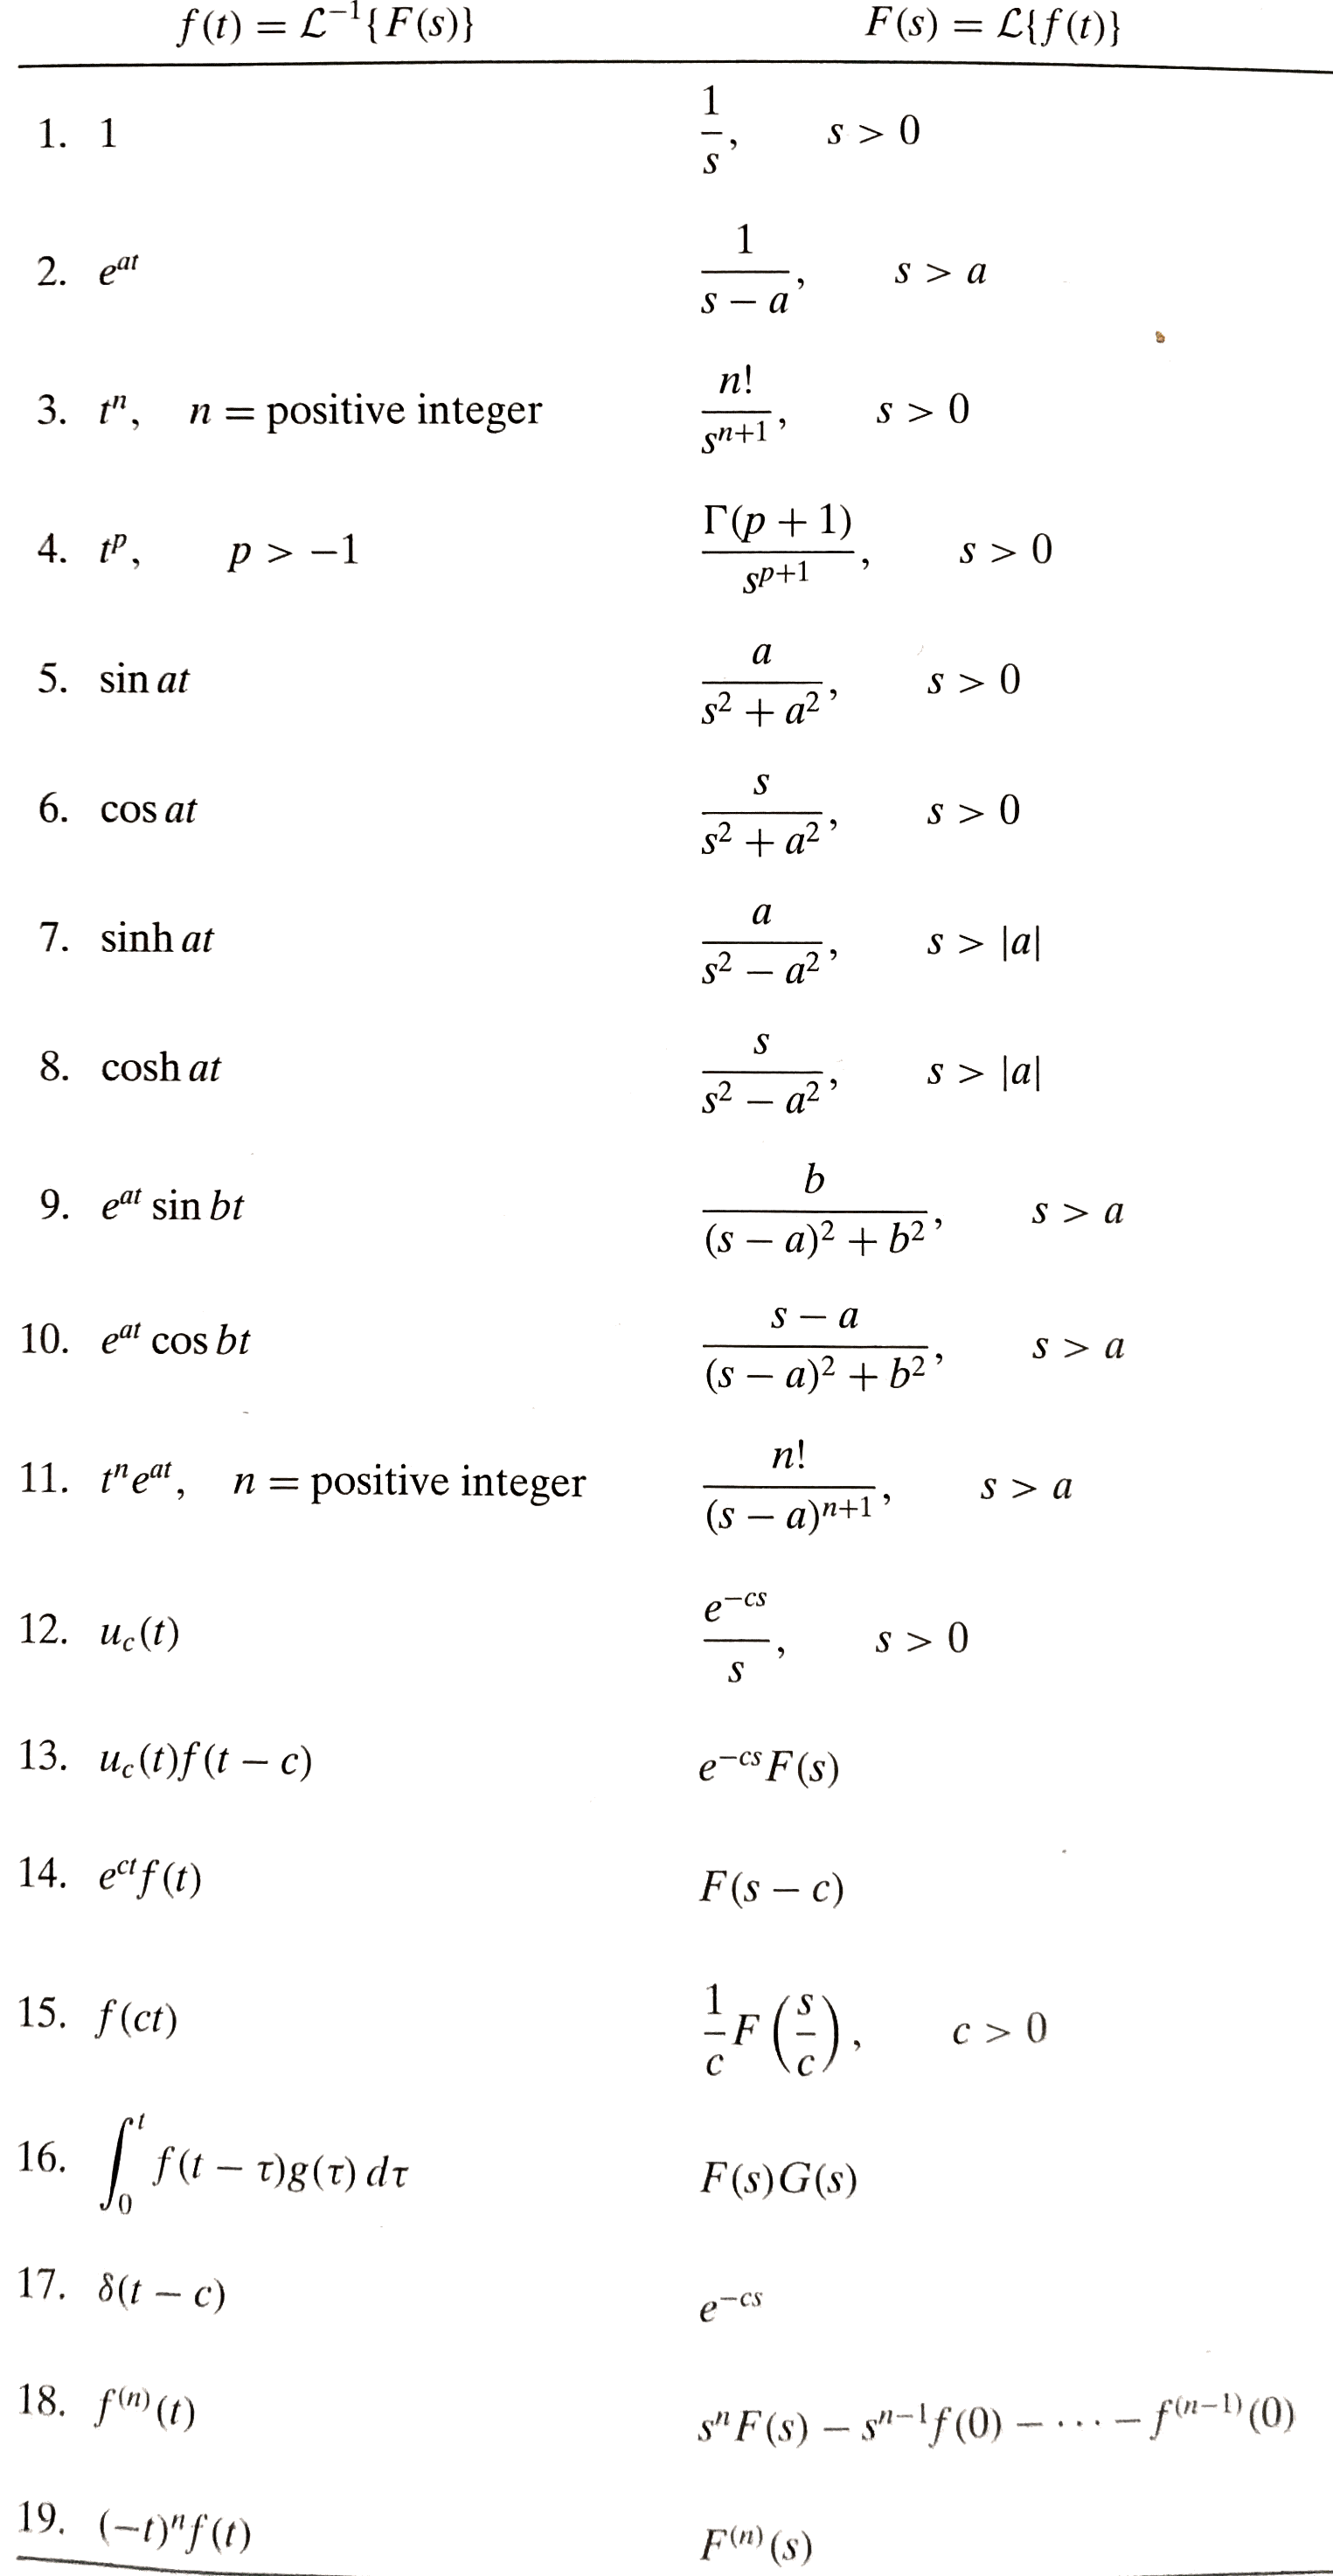
\includegraphics[width=0.9\columnwidth]{laplace}

\iffalse % NOT SHOWN
	\begin{tabular}{|c|c|}
	\hline
	$f(t) = \mathcal{L}^{-1}\{F(s)\} $ & $F(s) = \mathcal(L)\{f(t)\}$\\
	\hline 
	$1$       &  $\dfrac{1}{s}, \qquad s>0$ \\
	$e^{at}$ & $\dfrac{1}{s-a},  \qquad s>a$ \\
	$e^{at}f(t)$& $F(s-a)$	\\
	\end{tabular}
\fi % UP TO HERE (ended up scanning it to save time)

		\subsubsection{Unit Step Function}
		Given a function $f(t)$ defined for $t \geq0$, 
		$$ f(t)u_c(t) = \left\{
       		        \begin{array}{ll}
               		f(t) \quad \text{for}  \quad t\geq c\\
                  	0 \quad \text{for} \quad t < c
                		\end{array} \right. $$
                
              	$$ f(t)(u_a(t) -u_b(t)) = \left\{
                		\begin{array}{ll}
                  	f(t) \quad \text{for}  \quad t\in [a,b)\\
                  	0 \quad \text{for} \quad t \not\in [a,b)
                		\end{array} \right. $$
                
		\subsubsection{Dirac Distribution}
		$$ \delta(t) = 0 \quad \text{for} \quad t \neq 0, \quad \int_{-\infty}^{\infty} \delta(t)dt = 1 $$
		$$  \int_{-\infty}^{\infty} \delta(t - t_0)f(t)dt = f(t_0)$$

	\subsection{Convolution}
	Convolution is commutative, associative and distributive, but $(f*1) \neq f$ and $(f*f) \neq f^2$.
	$$ (f * g)(t) = \int_0^t f(\tau)g(t-\tau)d\tau $$
	$$ \mathcal{L} \{f*g\} = (\mathcal{L} \{f\})(\mathcal{L} \{g\}) $$

\section{First-Order Systems of ODEs}
$$x'_i(t) = F_i(x_j(t),t) \quad i,j=1,...,n$$

\iffalse % NOT SHOWN
	Fixed $t$ and $x_j$ - $\mathbf{F}(\mathbf{x},t)$ is a vector.\\
	Fixed $t$ and - $\mathbf{F}( ,t)$ is a vector field.\\
	Solution $\mathbf{x}(t) = (x_1(t),...,x_n(t)$ everywhere tangent to the vector field $\mathbf{F}$.
\fi % UP TO HERE		

		\subsubsection{From $n$-th order to system of first-order ODEs}
		$$y^{(n)} = F(y,y',...,y^{(n-1)},t)$$
		Change variables to $x_1 = y, x_2 = y',... , x_n = y^{(n-1)}$ and take derivatives $x'_1 = x_2, x'_2 = x_3,...,x'_{n-1}=x_n  $ and $x'_n = y^{(n)} = F(x_1,x_2,...,x_n,t)$. \\
		A first-order ODE system is linear if it has the form $$x'_i = \frac{dx_i}{dy} = \sum_{j=1}^nP_{ij}(t)x_j + g_i(t) \quad i =1,...,n$$


\section{Homogeneous Systems of Linear ODEs}
% A first-order ODE system is linear if it has the form $$x'_i = \frac{dx_i}{dy} = \sum_{j=1}^nP_{ij}(t)x_j + g_i(t) \quad i =1,...,n$$
% If $g_i(t) = 0$ it is homogeneous. 
% If $P_{ij}(t), g_i(t)$ are continuous in $t \in [\alpha,\beta]$ then $\exists$ unique solution $x_i = \phi_i(t)$ solving the IVP, i.e. $\phi_i(t_0) = x_i^0$. 
$$\frac{d\mathbf{x}}{dt} = P(t)\mathbf{x}$$
The general solution is given by the linear combination of any fundamental set of $n$ solutions 
    \vspace{-0.2cm}
$$ \mathbf{x}_{\text{gen}}(t) = \sum_{j=1}^n c_j\mathbf{x}_j(t)$$  $$\text{with} \quad
    W[\mathbf{x}_1,...,\mathbf{x}_n] = |\mathbf{x}_1, \mathbf{x}_2,...,\mathbf{x}_n| = \det \Psi(t) \neq 0. $$                                 
    
    \textbf{Liouville's Theorem}  
    $$\dot{W} = W \text{tr}P  \implies W(t) = e^{\int_{t_0}^t \text{tr} P(s)ds}W(t_0)$$
    
 		\subsubsection{Different Eigenvalues: Real}
  		We look for exponential solutions of $\frac{d\mathbf{x}}{dt} = A\mathbf{x}$ with $\mathbf{x} = e^{rt}\boldsymbol{\xi} \implies \frac{d\mathbf{x}}{dt} = r\mathbf{x}$. \\
  		If the corresponding eigenvalue problem $(A-r\mathbb{I})\boldsymbol{\xi} = 0$ has different eigenvalues $r_i$, the eigenvectors $\boldsymbol{\xi}^{(i)} $ are linearly independent and the general solution reads $$ \mathbf{x} = \sum_{j=1}^n c_j e^{r_jt}\boldsymbol{\xi}^{(j)}.$$
  		If an eigenvalue $r$ has algebraic multiplicity $s\geq 2$, the method still works if the geometric multiplicity (number of linearly independent eigenvectors) equals $s$.
  
   		\subsubsection{Different Eigenvalues: Complex}
    		If $r_1= \lambda + i\mu$ is and eigenvalue, i.e. $(A-r_1\mathbb{I})\boldsymbol{\xi}_1 = 0$ then the complex conjugate $r_1^* = \lambda - i\mu$ is also an eigenvalue with eigenvector $\boldsymbol{\xi}_1^*$. \\ 
    		To convert into real solutions, write $ \boldsymbol{\xi}_1 = \mathbf{a} + i\mathbf{b}$, then the 2 real solutions are 
		\begin{align*}
			\mathbf{u}(t) = e^{\lambda t} (\mathbf{a}\cos{\mu t} - \mathbf{b} \sin{\mu t} )\\
			\mathbf{v}(t) = e^{\lambda t} (\mathbf{a}\sin{\mu t} + \mathbf{b}\cos{\mu t} )
		\end{align*} and the general solution: $\mathbf{x}(t) = c_1\mathbf{u}(t) + c_2\mathbf{v}(t) +...$
  
  
 		\subsubsection{Fundamental Matrix}
  		A fundamental marix $\Psi(t)$ is an $n\times n$ matrix with fundamental solutions as columns: 
  		$$ \Psi(t) = \begin{pmatrix} 
       			 x_1^{(1)}    & \dots &  x_1^{(n)} \\
      			\vdots   & \ddots   &  \vdots \\
     			 x_n^{(1)}   & \dots & x_n^{(n)} \\ 
 			 \end{pmatrix} $$
		\begin{itemize}
  			\item $\det \Psi(t) = W(t) \neq 0$
			\item $ \mathbf{x}(t) = \sum_{j=1}^n c_j\mathbf{x}^{(j)} = \Psi(t)\mathbf{c}, \quad \mathbf{c} = (c_1,...,c_n)^T$.
			\item If $\mathbf{x}(t_0) = \Psi(t_0)\mathbf{c} = \mathbf{x}_0 \implies \mathbf{c} = \Psi^{-1}(t_0)\mathbf{x}_0$ \\ 
		 $ \mathbf{x}(t) = \Psi(t)\mathbf{c} = \Psi(t)\Psi^{-1}(t_0)\mathbf{x}_0$ (requires invertible $\Psi(t)$).
			\item $\Psi' = A\Psi$
		\end{itemize} 
		
  \textbf{Matrix exponential} 
  \begin{align*}
 	 e^{At} &= \sum_{n=0}^\infty \frac{(At)^n}{n!} = \mathbb{I}+At+\frac{1}{2!}A^2t^2+... \\
  	 &= \lim_{n \rightarrow \infty} \left(\mathbb{I}+\frac{1}{n}A\right)^n
  \end{align*}
  \begin{itemize}
  	\item $\mathbf{x}(t) = e^{At}\mathbf{x}_0 \iff e^{At} = \Psi(t)\Psi^{-1}(t_0)$
	\item$e^{At} = \Psi(t)$ for $\Psi(0) = \mathbb{I}$
  \end{itemize}
  
Let $\frac{d\mathbf{x}}{dt} = A\mathbf{x}$ and consider the matrix $T$ with eigenvectors $\boldsymbol{\xi}^{(i)}$ as columns. The matrix $AT$ has columns equal to $A\xi^{(1)} = r_i\xi^{(i)}$, so 
  \begin{align*}
  AT &= \begin{pmatrix} 
       r_1 \xi_1^{(1)}    & \dots &  r_n\xi_1^{(n)}   \\
      \vdots   & \ddots   &  \vdots \\
      r_1 \xi_n^{(1)}    & \dots & r_n \xi_n^{(n)}  \\
  \end{pmatrix} 
  = T \begin{pmatrix} 
        r_1  & 0& \dots &  0 \\
      	0 &  r_2 & \dots    & 0 \\
     	\vdots & \vdots & \ddots & \vdots \\
     	0 & 0 & \dots &r_n \\
  	\end{pmatrix} \\ &= T \text{diag}(r_1,...,r_n) = TD \implies D = T^{-1}AT .
  \end{align*}
  
Then $\mathbf{x} = T\mathbf{y} \implies \frac{d\mathbf{y}}{dt} = D\mathbf{y}$ and in the new variables, the solution is 
\vspace{-0.35cm}
$$\mathbf{y}_i = e^{r_it} \begin{pmatrix} 0 \\  . \\ 1 \\ 0 \\ . \\0 \end{pmatrix} \quad \text{1 $i$-th component.}$$

Thus its fundamental matrix equals $Q(t) = e^{Dt} = \text{diag}(e^{r_1t},...,e^{r_nt})$. 
The fundamental matrix in the original variables $\mathbf{x}$ is $\Psi(t) = TQ(t)$ and the exponential matrix is $e^{At} = \Psi(t)\Psi^{-1}(0) = TQT^{-1}$. Only works if $A$ is diagonalisable. If we have an eigenvalues with geometric multiplicity < algebraic multiplicity, we cannot diagonalise!

	\subsection{Repeated Eigenvalues}
	If the algebraic multiplicity > geometric multiplicity, then follow these steps:
	\begin{enumerate}
		\item One solution is $\mathbf{x}_1 = e^{\lambda t} \boldsymbol{\xi}$.
		\item Second solution is of the form $\mathbf{x}_2 = te^{\lambda t} \boldsymbol{\xi} + e^{\lambda t} \boldsymbol{\eta}$ with $ (A-\lambda \mathbb{I}) \boldsymbol{\eta} = \boldsymbol{\xi}$.
		\item (Third solution is of the form $\mathbf{x}_3 = \frac{t^2}{2}e^{\lambda t} \boldsymbol{\xi} + te^{\lambda t} \boldsymbol{\eta} + e^{\lambda t} \boldsymbol{\zeta}$ with $ (A-\lambda \mathbb{I}) \boldsymbol{\zeta} = \boldsymbol{\eta}$.)
	\end{enumerate}

	\textbf{Connection to matrix methods} Build a matrix $T$ out of $\boldsymbol{\xi}, \boldsymbol{\eta}, (\boldsymbol{\zeta})$, then $T^{-1}AT = J$ where $J$ is an upper triangular matrix (Jordan form). We can then proceed as if it was $D$ above. The exponential has the form 
	$$ e^{J_{\lambda}t} = \begin{pmatrix} e^{\lambda t} & te^{\lambda t} \\ 0 & e^{\lambda t} \end{pmatrix}. $$

\section{Nonhomogeneous Systems of ODEs}
$$ \mathbf{x}' = A\mathbf{x}+\mathbf{g}(t)$$
The general solution is of the form \[ \mathbf{x}(t) = \sum_i c_i\mathbf{x}^{(1)}(t) + \mathbf{x}_{\text{par}}(t). \]

	\subsubsection{Diagonalisation}
	Introduce change of variables $\mathbf{x}=T\mathbf{y}$, so we have
	$$ T\mathbf{y}' = AT\mathbf{y} + \mathbf{g}(t) \implies \frac{d\mathbf{y}}{dt} = D\mathbf{y} + T^{-1}\mathbf{g} = D\mathbf{y}+\mathbf{h}.$$
	This leads to a system of $n$ decoupled equation which we solve by direct integration:
	$$ y'_i = r_iy_i + h_i \implies y_i(t) = c_i e^{r_i t} + e^{r_i t}\int_{t_0}^t e^{-r_is}h_i(s)ds.$$
	General solution in the original variables equals $\mathbf{x}(t) = T\mathbf{y}(t)$.
	In case the matrix is not diagonalisable, find its Jordan form and proceed in a similar way (with $J$ instead of $D$). Note that we will need to integrate from the bottom up. 

		\subsubsection{Method of Undetermined Coefficients}
		Works if $\mathbf{g}(t)$ is built out of polynomials and exponentials (real or complex). Same rules apply with the exception that if $\mathbf{g}(t) = \mathbf{u}e^{\lambda t}$ where $\lambda$ is an eigenvalue of $A$ with multiplicity 1, then $$ \mathbf{x}_{\text{par}} = te^{\lambda t}\mathbf{a}+e^{\lambda t} \mathbf{b}. $$
		If the multiplicity is $n$, we must write $\mathbf{x}_{\text{par}} = e^{\lambda t}\sum_{i=0}^n t^i \mathbf{a}_i.$

		\subsubsection{Variation of Parameters}
		If $A = P(t)$ is not constant, we look for solutions to the non-homogeneous part of the form $$ \mbf{x}(t) = \Psi(t)\mbf{u}(t).$$ Introducing this to the system gives $$ \f{d\mbf{x}}{dt} = \Psi'(t)\mbf{u}(t) +\Psi(t)\f{d\mbf{u}}{dt} = P(t)\Psi(t)\mbf{u}(t)+\mbf{g}(t).$$
 		Remembering $\Psi' = P(t)\Psi$, $$ \Psi \f{d\mbf{u}}{dt} = \mbf{g}(t) \implies \f{d\mbf{u}}{dt} = \Psi^{-1}\mbf{g} \implies \mbf{u}(t) = \int_{t_0}^t \Psi^{-1}(s)\mbf{g}(s)ds +\mbf{f}$$
 		Thus the general solution is $$ \mbf{x}(t) = \Psi(t)\Psi^{-1}(t_0)\mathbf{x}_0 + \Psi(t)\int_{t_0}^t \Psi^{-1}(s)\mbf{g}(s)ds.$$
 
 \section{Qualitative Theory of ODEs}
 Consider a nonlinear autonomous system (i.e. $F,G$ have no explicit time dependence) $$ \f{dx}{dt} = F(x,y), \quad  \f{dy}{dt} = G(x,y).$$

 	\subsection{Critical Points} 
	A point $\mbf{x}_0 =(x_0,y_0)$ is a critical point if $F(x_0,y_0) = G(x_0,y_0) = 0$.
 	Locally, around any critical point, nonlinear ODEs $\approx$ linear ODEs. Use Taylor expansions (for $F$ and $G$):
 	\begin{align*} 
		F(x,y) = F(x_0,y_0) + \partial_x F(x_0,y_0)(x-x_0)\\ + \partial_y F(x_0,y_0)(y-y_0) +  \eta_1(x,y)
	\end{align*}
	where $\f{\eta_1(x,y)}{||\mbf{x}-\mbf{x_0}||} \rightarrow 0$ as $(x,y) \rightarrow (x_0,y_0)$. Linear approximation consists of dropping $\eta_1$. \\
	Introduce new variables $u_1 \equiv x-x_0$,  $u_2 \equiv y-y_0$. These satisfy 
	$$ \f{d\mbf{u}(t)}{dt} = 
	\begin{pmatrix}
		 \partial_x F(x_0,y_0) & \partial_y F(x_0,y_0) \\
		 \partial_x G(x_0,y_0) & \partial_y G(x_0,y_0)
	 \end{pmatrix} \begin{pmatrix} u_1 \\ u_2 \end{pmatrix} =  A\mbf{u}.$$
$A$ is the Jacobian matrix.
 
 	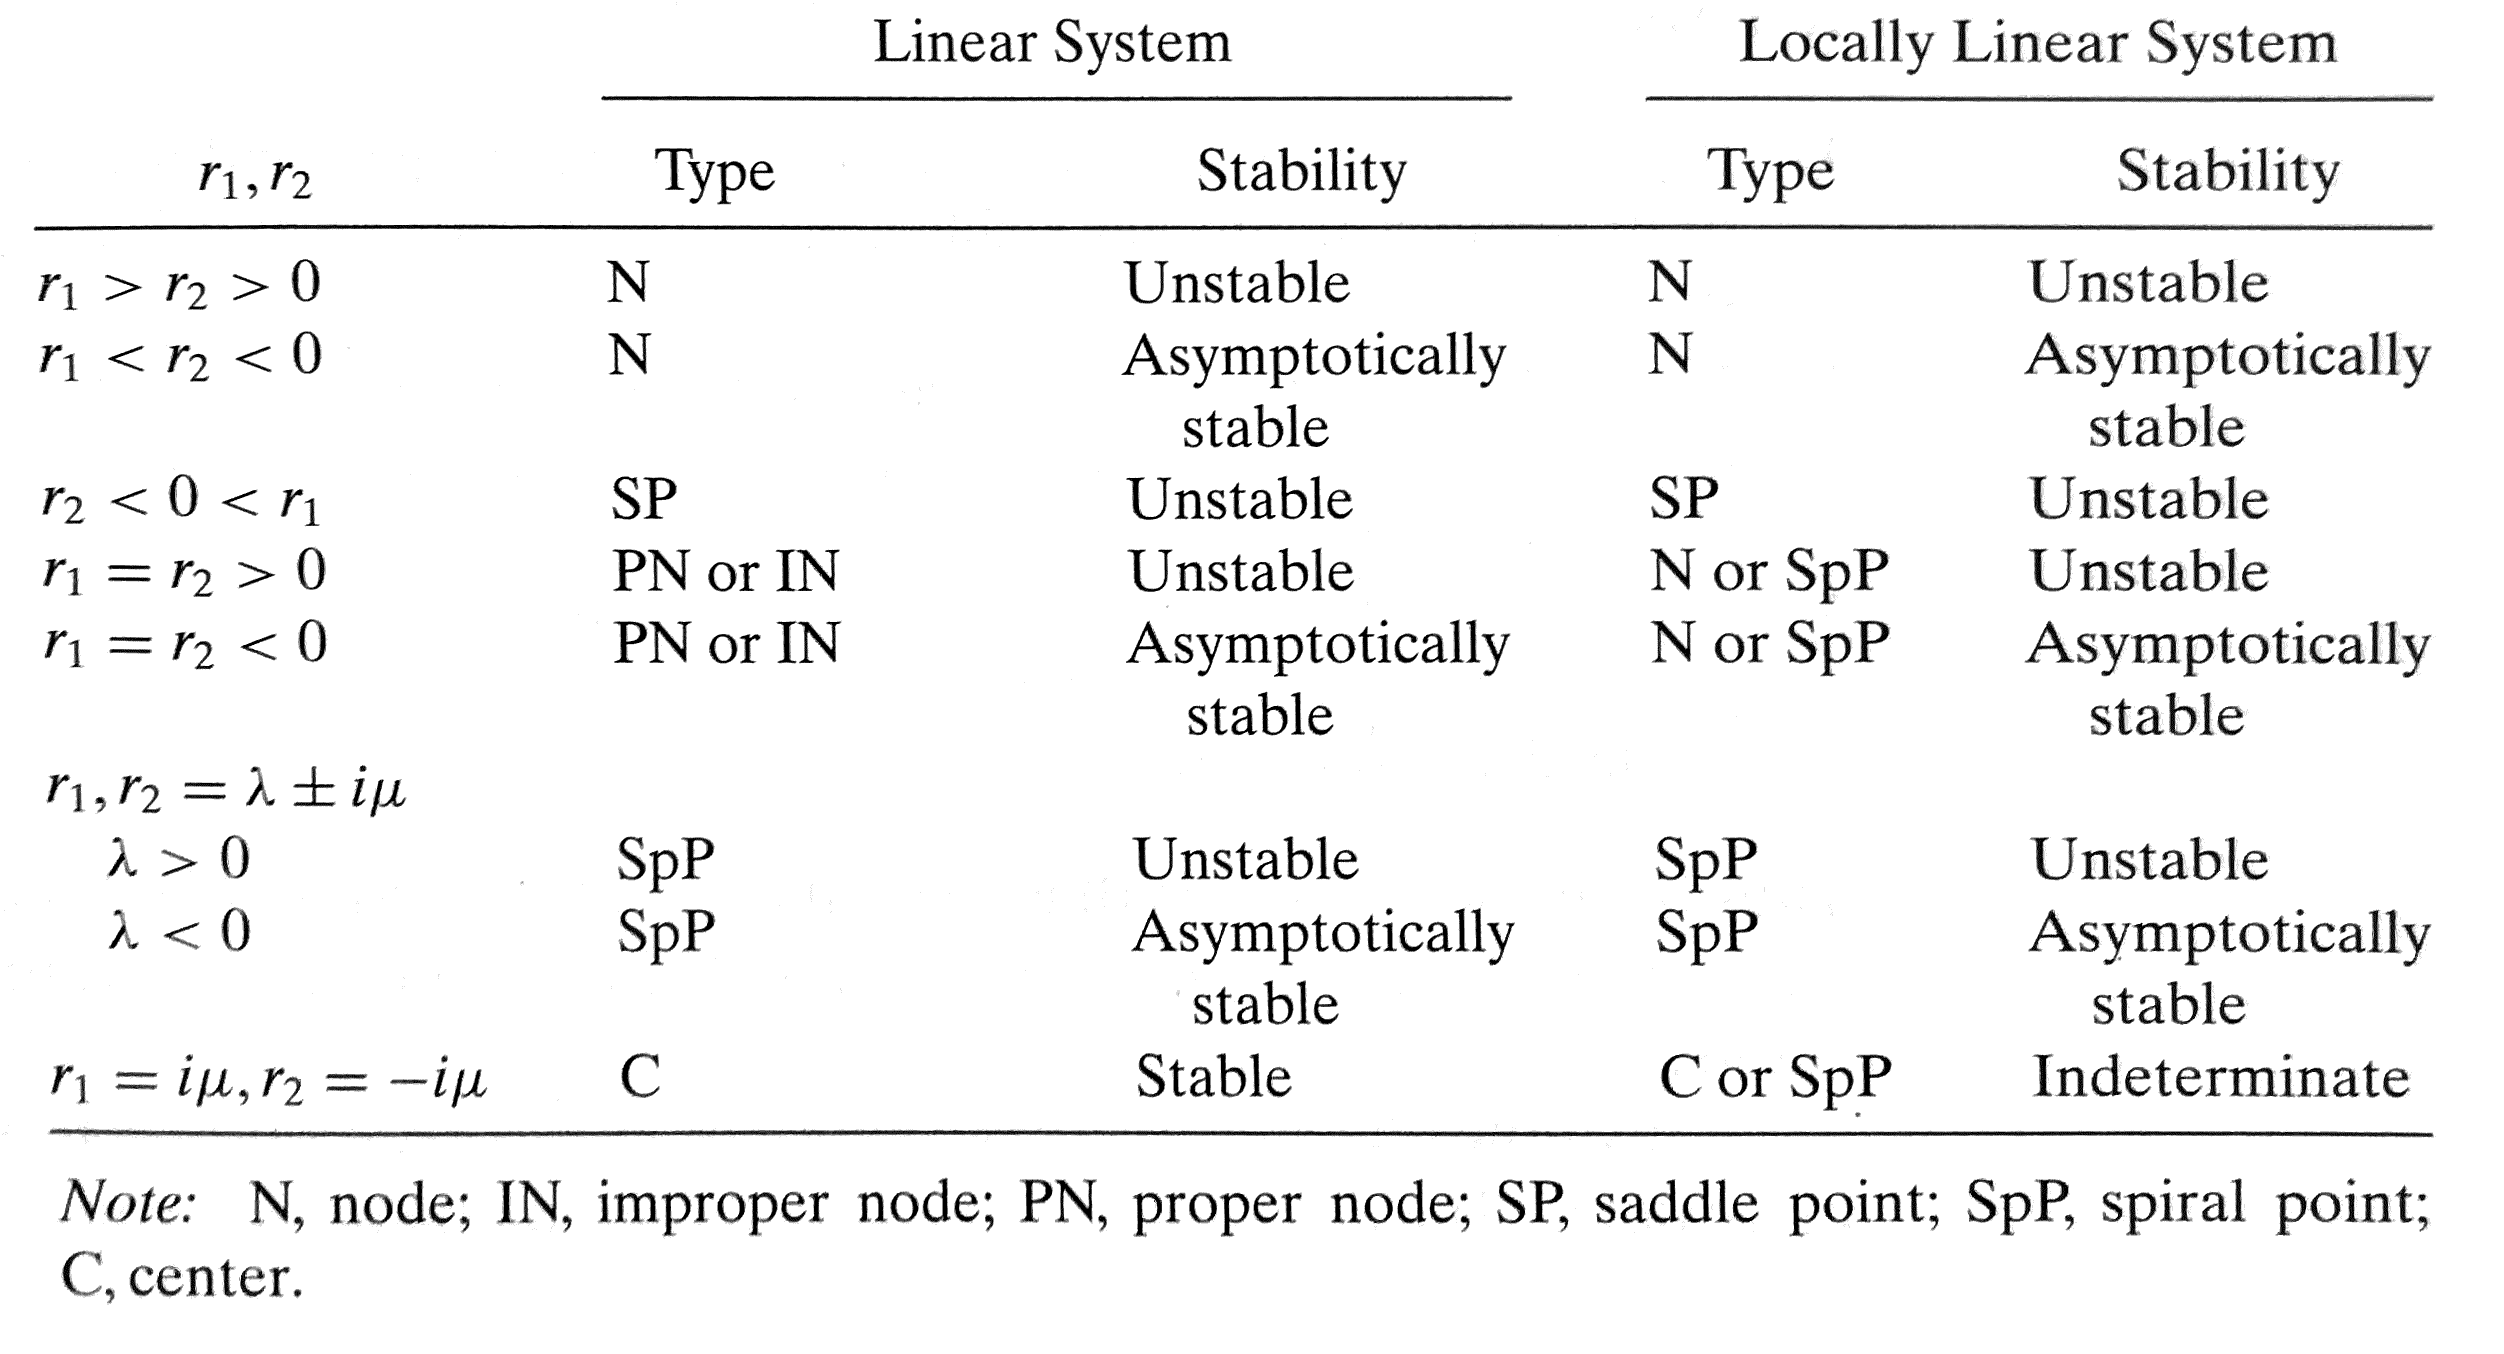
\includegraphics[width=1.0\columnwidth]{table}
 	A node is proper if it has independent eigenvectors and improper if there is a missing eigenvector.
	 A critical point $\mbf{x}_0$ is stable if $\forall \epsilon$, $\exists \delta>0$ s.t. every solution $\mbf{x} = \phi(t)$ with $||\phi(0)-\mbf{x}_0|| < \delta$ at $t=0$ satisfies $||\phi(t)-\mbf{x}_0|| < \epsilon$, $\forall t >0$.\\
	 A critical point $\mbf{x}_0$ is asymptotically stable if it is stable and the solution $\mbf{x} = \phi(t)$ is forced to approach $\mbf{x}_0$ as $t \rightarrow \infty$.
 
	Sometimes a nonlinear ODE system has an exact phase portrait given by 
 	\vspace{-0.2cm}
  	$$ \left. \begin{array}{ll}
		\f{dx}{dt} = F(x,y) \\ \f{dy}{dt} = G(x,y)
                \end{array}
              \right\} \implies \f{dy}{dx} = \f{G(x,y)}{F(x,y)} \implies H(x,y) = c. $$
  
  \iffalse % NOT SHOWN
  \subsection{Prey-Predator Model}
  \begin{align*}  \dot{x} &= ax-\alpha xy \\ \dot{y} &= -cy+\gamma xy \end{align*}
  ($x$ = prey, $y$ = predator, $a$ = growth rate of prey, $c$ = death rate of predator; all parameters are positive)
  \fi % UP TO HERE
  
  	\subsection{Lyapunov's Theory}
	 Let $E(x,y)$ be defined on a domain $D$ containing (0,0). \\
 	$ E(x,y)$ is \emph{positive (negative) definite} if  $ E(0,0) = 0$ and  $ E(x,y) >0$ $\forall(x,y)\in D$ ($ E(x,y) < 0$ $\forall(x,y)\in D$). \\
  	$ E(x,y)$ is \emph{positive (negative) semi-definite} if  $ E(0,0) = 0$ and  $ E(x,y) \geq 0$ $\forall(x,y)\in D$. ($ E(x,y) \leq 0$ $\forall(x,y)\in D$.  \\
	
  	\textbf{Theorem} Given an autonomous system with critical point (0,0), if $\exists E(x,y)$ continuous with continuous first partial derivatives, positive definite and for which $\f{dE}{dt}$ is negative definite on some domain $D$ containing (0,0) then (0,0) is asymptotically stable. If $\f{dE}{dt}$ is negative semi-definite $\implies$ (0,0) is stable (at the non-linear level). $E(x,y)$ is called \emph{Lyapunov function}. \\
  
   	\textbf{Theorem } Given an autonomous system with critical point (0,0), assume $\exists E(x,y)$ continuous with continuous first partial derivatives, such that $E(0,0) = 0$ and that in every neighbourhood of (0,0) $\exists$ at least one point $(x_1,y_1)$ where $E(x_1,y_1)$ is positive (negative). If $\exists$ some domain $D$ containing (0,0) where $\f{dE}{dt}$ is positive definite (negative definite) on $D \implies$ (0,0) is an unstable critical point.
    
    	\subsection{Limit Cycles}
	Periodic solutions: $f(x+T) = f(x)$ $\forall x$ (the smallest possible $T$ is fundamental period). Trajectories form closed curves. 
	A linear combination or product of functions with the same period $T$ also have period $T$. \\Limit cycles are periodic solutions s.t. at least one other non-closed trajectory asymptotes to them as $t\rightarrow  \infty$ (or $-\infty$ or both). \\
	Let $F(x,y), G(x,y)$ have continuous first partial derivatives in some domain $D$. The we have the following:\\
	
     	\textbf{Theorem}  A closed trajectory must necessarily enclose at least one critical point. If it encloses only one critical point, it cannot be a saddle point. (i.e. no critical points in $D \implies$ no closed trajectories in $D$; if $\exists$ a unique critical point in $D$ and it is a saddle $\implies$ no closed trajectories in $D$).\\
	
        \textbf{Theorem} Let $D$ be simply connected (i.e. without holes). If $\partial_xF + \partial_yG$ has the same sign in $D \implies$ there are no closed trajectories in $D$.\\
        
        \textbf{Poincar\'e-Bendixon Theorem} Let $R$ consist of a bounded subdomain of $D$ and its boundary. Suppose $R$ has no critical points. If a certain trajectory lies entirely in R, then this trajectory either is a periodic (closed) trajectory or spirals towards one. Either way,  $\exists$ a closed trajectory.
           
\section{Fourier Series}  
	\textbf{Inner Product}  
	\begin{align*}
		(u(x),v(x)) &\equiv \int_{-L}^L u(x)v(x)dx \\
		(u(x),v(x)) &\equiv \int_{\alpha}^{\beta} u^*(x)v(x)dx \quad \text{ (complex functions)} 
        \end{align*}
        The set $ \{1,  \sin{\f{n \pi x}{L}}, \cos{\f{m \pi x}{L}} \} $ forms an orthogonal basis. If $S_n(x) = \sin{\f{n \pi x}{L}}, S_m(x) = \sin{\f{m \pi x}{L}}, C_n(x) = \cos{\f{n \pi x}{L}}, C_m(x) = \cos{\f{m \pi x}{L}}, C_0 = 1$, then 
        \begin{align*}
        		\left. \begin{array}{ll}
			(S_m,S_n) &= 0  \\
          		(S_n,S_n)&= L 
                \end{array}
              \right\} \implies (S_m,S_n) = L \delta_{mn} \quad m,n \neq 0 \\
          	\left. \begin{array}{ll}
			(C_m,C_n) &= 0 \\
           		(C_n,C_n) &= L 
                \end{array}
              \right\} \implies (C_m,C_n) = L \delta_{mn} \quad m,n \neq 0 \\
	(S_m,C_n) = (S_n, C_n) = (C_0,C_m) = (C_0,S_m) = 0, \quad (C_0,C_0) = 2L. \end{align*}

	A periodic function with period $2L$ can be expressed as \emph{Fourier series} 
	\begin{align*} 
		f(x) &= \f{a_0}{2} + \sum_{n=1}^{\infty} \left( a_n \cos{\f{n \pi x}{L}} + b_n \sin{\f{n \pi x}{L}} \right) \\
		 &= \sum_{n = - \infty}^{\infty} c_n e^{i n \pi x / L} 
	\end{align*}

	For piecewise continuous functions the series converges to $f(x)$ $\forall x$ where $f(x)$ is continuous. At discontinuities, the series converges to $ \f{f(x^+)+f(x^-)}{2}$, not to $f(x)$ - Gibbs phenomenon.

		\subsubsection{Euler-Fourier Formulas} Projecting the function onto orthogonal basis gives 
		\begin{align*} 
			\f{a_0}{2} &= \f{1}{2L} \int_{-L}^L f(x) dx \equiv \langle f(x) \rangle = c_0\\
   		        a_n  &= \f{1}{L} \int_{-L}^L f(x) \cos{\f{n \pi x}{L}} dx, \quad n=0,1,2,... \\
   		        b_n &= \f{1}{L} \int_{-L}^L f(x) \sin{\f{n \pi x}{L}} dx \\
    		        c_n &= \f{a_n - ib_n}{2}, \quad c_{-n} =  \f{a_n + ib_n}{2} \quad (n>0) \\
   		        c_n &=  \f{1}{2L} \int_{-L}^L f(x)e^{-\f{i n \pi x}{L}}dx, \quad n \in \mathbb{Z}
		\end{align*}

		Even functions ($f(-x)=f(x)$) only have cosine coefficient series. Odd functions ($f(-x) = -f(x)$) only have sine coefficient series. Due to symmetries, even/odd functions only require information about half the interval $[0,L]$.

		\subsubsection{Parseval's Theorem}
		\begin{align*}
			(f,f) &= \int_{-L}^L |f(x)|^2 dx = 2L \sum_{n = - \infty}^{\infty} |c_n|^2 \\
			 &= L \left[ \f{|a_0|^2}{2} + \sum_{n=1}^{\infty} (|a_n|^2 + |b_n|^2) \right] 
 		\end{align*}

\section{Partial Differential Equations}
 \begin{itemize}
 	\item Assume separation of variables $u(x,t) = X(x)T(t)$.
	\item Introduce one (or more) separation parameter $\lb$.
	\item Solve eigenvalue problem(s): quantisation of $\lb$ (depends on boundary / initial conditions).
	\item Write the most general solution as a linear combination of all solutions to the eigenvalue boundary problems.
	\item Identify any undetermined coefficients using initial conditions.
 \end{itemize}
 
		\subsubsection{Heat Equation}
		$$ \partial_t u =\alpha^2 \partial_x^2 u, \quad \alpha > 0 $$
		\begin{itemize}
			\item initial condition: $u(x,0) = f(x)$, $0\leq x \leq L $\\
			\item boundary conditions: $u(0,t), u(L,t)$, $t >0$ 
		\end{itemize}
		
		\textbf{Homogeneous boundary conditions} $u(0,t) =  u(L,t) = 0$
		\begin{align*}
			u(x,t) = X(x)T(t) \implies X''+\lb X &= 0 \\ T'+\alpha^2 \lb T &= 0 
		\end{align*}
		\begin{align*}
			X_n(x) &= \sin{\f{n \pi x}{L}}, \quad n=1,2,3,... \quad \lb_n = \f{n^2 \pi^2 }{L^2} \\
			T_n &= e^{-\f{n^2 \pi^2 \alpha^2 t}{L^2}}
		\end{align*}
		$$ u(x,t) = \sum_{n=1}^{\infty} c_nX_n(x)T_n(t) = \sum_{n=1}^{\infty} c_n e^{-\f{n^2 \pi^2 \alpha^2 t}{L^2}} \sin{\f{n \pi x}{L}} $$
		$$ c_n = \f{2}{L} \int_0^L f(x)  \sin{\f{n \pi x}{L}} dx $$

		\textbf{Nonhomogeneous boundary conditions} $u(0,t) =  T_1, u(L,t) = T_2$. \\
		Map problem to one with homogeneous boundary conditions. Define time independent function $g(x) = \lim_{t \rightarrow \infty}u(x,t).$ 
		$$g(x) = T_1 +(T_2-T_1)\f{x}{L} \implies u(x,0) = f(x)-g(x)$$

		Then $\partial_t g = 0$ and it is easy to solve for $g(x)$. The original problem has the form $u(x,y) = g(x) + w(x,t)$ ($w(x)$ satisfies a homogeneous set of boundary conditions with different initial value function). 
		$$ c_n = \f{2}{L} \int_0^L (f(x)-g(x))  \sin{\f{n \pi x}{L}} dx$$
		$$ u(x,t)  = T_1 + (T_2-T_1)\f{x}{L}  + \sum_{n=1}^{\infty} c_n e^{-\f{n^2 \pi^2 \alpha^2 t}{L^2}} \sin{\f{n \pi x}{L}} $$

		\textbf{Insulated ends} $X'(0) = X'(L) = 0$ \\ Process is the same but this time the result is a cosine series. 

		\subsubsection{Wave Equation}
		$$\partial_t^2 u = a^2 \partial_x^2 u \quad \text{ $a$ = wave speed}$$
		\begin{itemize}
			\item initial position: $u(x,0) = f(x)$ \\
			\item initial velocity $u_t(x,0) = g(x)$ \\
			\item fixed ends: $u(0,t) = u(L,t) = 0 $ 
		\end{itemize}
		
		\textbf{String with initial position} No initial velocity, so $u_t(x,0) = 0 \implies T'(0) = 0$. $X_n$ and $c_n$ are same as homogeneous heat equation.
		$$ u(x,t) = \sum_{n=1}^{\infty} c_nX_n(x)T_n(t) = \sum_{n=1}^{\infty} c_n \sin{\f{n \pi x}{L}} \cos{\f{n \pi a t}{L}} $$

		\textbf{String with initial velocity} No initial position, so $u(x,0) = 0 \implies T(0) = 0$. We find that $$ T_n(t) = \sin{\f{n \pi a t}{L}}$$
		$$ u(x,t) = \sum_{n=1}^{\infty} c_n \sin{\f{n \pi x}{L}} \sin{\f{n \pi a t}{L}} $$
		$$ c_n = \f{2}{n \pi a} \int_0^L g(x)  \sin{\f{n \pi x}{L}} dx $$

		\textbf{String with initial position and velocity} Let $v(x, t)$ be the solution for the vibrating string with no initial velocity ($g(x) = 0$). Let $w(x, t)$ be the solution for the string with no initial displacement ($f(x) = 0$). Then $u(x, t) = v(x, t) + w(x, t).$

		\subsubsection{Laplace's Equation}
		$$ \nabla^2u \equiv \partial_x^2 u + \partial_y^2 u = 0 $$
		Dirichlet boundary conditions: $u(x,y)$ specified at the boundary. \\
		
		\textbf{Rectangle} Assume separation of variables $u(x,y) = X(x)Y(y)$. Then 
		\begin{align*}
			X'' - \lb X = 0 \\
			Y'' + \lb Y = 0 
		\end{align*}
		Example : $u(x,0)=u(x,b)=0, u(0,y) =0, u(a,y) = f(y), 0 \leq x \leq a, 0 \leq y \leq b$
		$$ u(x,y) =  \sum_{n=1}^{\infty} c_n \sinh{\f{n \pi x}{b}} \sin{\f{n \pi y}{b}} $$
		$$ c_n  \sinh{\f{n \pi a}{b}}  = \f{2}{b} \int_0^b f(y)  \sin{\f{n \pi y}{b}} dy $$

		\textbf{Disc} Change coordinates:
		$$ \f{\partial^2 u }{\partial r^2} + \f{1}{r^2}\f{\partial^2u}{\partial \theta^2} + \f{1}{r}\f{\partial u }{\partial r} = 0$$
		Assume $u(r,\theta) = R(r)\Theta(\theta)$, then 
		\begin{align*}
			r^2R'' +rR' = \lb R \\
			\Theta'' =  -\lb \Theta
		\end{align*}
		Example: $u(a,\theta) = f(\theta), x^2 + y^2 = a^2, 0 \leq \theta \leq 2\pi$ and $u(x,y) = \sqrt{x^2 + y^2} \leq a$ \\
		Periodicity and boundedness determine:
		\begin{itemize}
			\item $\lb = 0$ allows a constant solution $u_0(r,\theta) = \f{c_0}{2}$.
			\item $\lb = n^2$ allows solutions of the form $u_n(r,\theta) = r^n (a_n \cos{n\theta} + b_n \sin{n\theta})$
		\end{itemize}
		$$ u(r,\theta) = \f{c_0}{2} + \sum_{n=1}^{\infty} r^n(e_n\cos{n\theta} + f_n \sin{n\theta} )$$
		$$ u(a,\theta) = f(\theta) =  \f{c_0}{2} + \sum_{n=1}^{\infty} a^n(e_n\cos{n\theta} + f_n \sin{n\theta} )$$
		$$ a^n e_n = \f{1}{\pi} \int_{-\pi}^{\pi} f(\theta)\cos{n\theta} d\theta $$
		$$ a^n f_n = \f{1}{\pi} \int_{-\pi}^{\pi} f(\theta)\sin{n\theta} d\theta $$

           
	\subsection{Sturm-Liouville Boundary Problems}
		\subsubsection{Homogeneous Problems}
		Consider differential equations of the form $$[ p(x)y']' - q(x)y + \lb r(x)y = 0 $$
		Define the differential operator $L$ and rewrite the equation 
		\begin{align*}
			L[y] &= -[ p(x)y']'  + q(x)y \\
			L[y] &= \lb r(x)y 
		\end{align*}
		$$a_1 y(0)+a_2y'(0) = 0 \quad b_1y(1) + b_2 y'(1) = 0$$
		All eigenvalues $\lb$ for which there are nontrivial solutions are real. If we have two eigenvalues $\lb_1$ and $\lb_2$ with $\lb_1 \neq \lb_2$ and corresponding eigenfunctions $\phi_1, \phi_2$ then 	$$ \langle \phi_1, \phi_2 \rangle = \int_0^1 r(x)\phi_1(x)\phi_2(x) dx = 0. $$
		That is, the pair is orthogonal with respect to the inner product defined by the Sturm-Liouville problem (w.r.t the weight function $r(x)$), denoted by the angled brackets to differentiate from the original inner product.  For each eigenvalue, there is a unique linearly independent eigenfunction. They form and infinite ordered sequence $\lb_1 < \lb_2 .. < \lb_n$ and $\lb_n \rightarrow \infty$. \\
		Eigenfunctions satisfying $$ \langle \phi_n, \phi_n \rangle = \int_0^1 r(x)\phi_n^2 (x) dx = 1 $$ are said to be normalised and form an orthonormal set w.r.t. $r(x)$. 
		A function$f(x)$ can be written as a sum of these eigenfunctions as follows:
		$$ f(x) = \sum_{n=1}^{\infty} c_n \phi_n(x) $$
		Multiplying by $r(x)\phi_m(x)$ and integrating gives
		$$ \sum_{n=1}^{\infty} c_n  \int_0^1 r(x)\phi_m(x)\phi_n(x) dx = c_m $$
		$$ c_m = \int_0^1 r(x)\phi_m(x)f(x) dx= \langle f(x), \phi_m \rangle $$

		
\textbf{Lagrange's Identity} $$ \int_0^1 (L[u]v - uL[v]) dx = [-p(x)(u'(x)v(x) - u(x)v'(x))]_0^1 = 0$$
$$  (L[u],v) -(u,L[v]) = 0 $$

		\subsubsection{Nonhomogeneous Problems}
		$$ L[y] = -[ p(x)y']'  + q(x)y = \mu r(x)y + f(x) $$
		First look at the homogeneous problem $L[y] = \lb r(x)y$ with eihenvalues $\lb_1,\lb_2..$ and eigenfunctions $\phi_1,\phi_2...$ Assume the solution $y= \phi(x)$ can be written as 
		\begin{align*}
			\phi(x) &= \sum_{n=1}^{\infty} b_n\phi_n(x) \\
			c_n &= \int_0^1 f(x)\phi_n(x)dx \\
			b_n &= \f{c_n}{\lb_n - \mu} \\
			y &= \phi(x) = \sum_{n=1}^{\infty} \f{c_n}{\lb_n - \mu}\phi_n(x)
		\end{align*}
		If $c_n$ is zero then $b_n$ is arbitrary - infinitely many solutions. If $\lb_n = \mu$ for some $n$ and $c_n \neq 0 $ then there are no solutions. \\
		Example: generalised heat equation $$ r(x)u_t = (p(x)u_x)_x - q(x)u +F(x,t) $$
with two boundary conditions $u_x(0,t)-h_1(0,t) =0, u_x(1,t)+h_2u(1,t) = 0$ and initial condition $u(x,0) = f(x).$
		Assume solution of the form \[ u(x,t) = \sum_{n=1}^{\infty} b_n(t)\phi_n(x) \] where $\phi_n$ are eigenfunctions of the problem. Expand $F(x,t)$ in the same basis. It is convenient to consider $$ \f{F(x,t)}{r(x)} = \sum_n \gamma_n(t) \phi_n(x) $$ $$ \text{with} \quad \gamma_n(t) = \int_0^1 r(x)  \f{F(x,t)}{r(x)}  \phi_n(x) dx = (F, \phi_n) $$
		Substituting we find $$ \dot{b_n} + \lb_nb_n(t) = \gamma_b(t) \quad n=1,2,3...$$
		Using initial conditions $$ u(x,0) = f(x) = \sum_n \alpha_n\phi_n(x) \implies \alpha_n = \int_0^1 r(x)f(x)\phi_n(x) dx $$
		$$ b_n(t) = \alpha_n e^{\lb_n t} + \int_0^t e^{-\lb_n(t-s)}\gamma_n(s) ds $$

		\subsubsection{Wave equation in 2D}
		
		\textbf{Rectangle} $$\partial_t^2 u = a^2 (\partial_x^2 u +\partial_y^2 u)  $$
		Separation of variables gives rise to:
		\begin{align*}
		 \f{X''}{X} + \f{Y''}{Y} = \f{T''}{a^2T} &= -(\lb + \mu) \\
			X'' + \lb X &= 0 \\ 
			Y'' + \mu Y &= 0
		\end{align*}
		Example : $0 \leq x \leq L, 0 \leq y \leq M$ with $u(0,y) = u(L,y) = u(x,0) = u(x,M) =0$.
		\begin{align*}
			X &= \sin(m\pi x /L), \quad \lb_m=m^2\pi^2 /L^2m \quad m=1,2,... \\
			Y &= \sin(n\pi y /M), \quad \mu_n=n^2\pi^2 /M^2m \quad n=1,2,... \\
			&T'' +a^2(\lb_m + \mu_n)T = 0 \\
			T(t) &= T_{mn}(t) = c_{mn}\cos(\omega_{mn} t) + d_{mn}\sin(\omega_{mn} t) 
		\end{align*} where $ \omega_{mn} = a\pi \sqrt{m^2/L^2 + n^2/M^2}$.\\
		General solution is $u(x,y,t) = X(x)Y(y)T(t)$.
		\begin{align*}
			u(x,y,0) &= f(x,y) = \sum_{m,n} c_{mn} \sin(m\pi x / L)sin(n \pi y / M)\\
			\partial_t u(x,y,0) &= g(x,y) = \sum_{m,n} d_{mn} \sin(m\pi x / L)\sin(n \pi y / M) \
		\end{align*}

		\textbf{Disc} \\
		$$ \partial_t^2 u = a^2 \left(\partial^2_r + \f{1}{r} \partial_r + \f{1}{r^2} \partial^2_{\theta}\right)u $$
		Separation of variables gives rise to:
		\begin{align*}
			\Theta'' + m^2\Theta = 0 \\
			T'' + a^2\mu^2T=0 \\
			R'' + \f{R'}{r} + \left( \mu^2 - \f{m^2}{r^2} \right) R = 0 
		\end{align*}
		Example: $ 0 \leq x^2 + y^2 \leq 1$ with $u(1,\theta,t) = 0, \partial_t u(x,y,0) = 0, u(r,\theta,0) = f(r,\theta).$ \\
		\begin{align*}
			T(t) &=k_1 \sin(\mu at) + k_2 \cos(\mu at) \\
			\Theta(\theta) &= a_1 \cos(m\theta) + a_2 \sin(m\theta) \\
			R(r) &= c_1J_m(\mu r) + c_2 Y_m(\mu r)
		\end{align*}
		Periodicity in $\theta$ requires $m=1,2,...$. Boundedness imposes $a_2 = 0$. $u(1,\theta,t)$ imposes $J_m(\mu) = 0$, i.e. $\mu = \mu_{m1}, \mu_{m1}...$ are zeroes of the Bessel function. Initial condition $\partial_t u(r,\theta,0) = 0$ imposes $k_1=0$. So the general solution is 
		\begin{align*}
			u &= \sum_m \sum_n (c_{mn}\cos(m\theta) + d_mn \sin(m\theta))\cos(a\mu_{mn}t)J_m(\mu_{mn} r) \\
			c_{mn} &\propto \int_0^1 \int_0^{2\pi} f(r,\theta) \cos(m\theta) J_{mn}(\mu_{mn}r)r dr d\theta \\
			d_{mn} &\propto \int_0^1 \int_0^{2\pi} f(r,\theta) \sin(m\theta) J_{mn}(\mu_{mn}r)r dr d\theta 
		\end{align*}

		\subsubsection{Third Laplace's Equation in Cylindrical Coordinates}
		$$ \nabla^2u \equiv \partial_x^2 u + \partial_y^2 u  +  \partial_z^2 u= 0 $$
		$$ \f{1}{\rho} \f{\partial}{\partial \rho} \left(\rho \f{\partial u}{\partial \rho} \right) + \f{1}{\rho^2} \f{\partial^2 u}{\partial \psi^2} + \f{\partial^2 u}{\partial z^2} = 0 $$
		Using separation of variables $u(\rho, \psi,z) = R(\rho)\Psi(\psi)Z(z)$,
		$$ \f{1}{R\rho} \f{d}{d \rho} \left(\rho \f{ dR}{d \rho} \right) + \f{1}{\rho^2 \Psi} \f{d^2 \Psi}{d \psi^2} + \f{1}{Z} \f{d^2 Z}{d z^2} = 0 $$
		\begin{align*}
			\f{d^2 Z}{d z^2} = \chi^2 Z \\
			\f{d^2 \Psi}{d \psi^2} = -m^2 \Psi \\
			\f{d^2R}{d\rho^2} + \f{1}{\rho} \f{dR}{d\rho} + \left( 1 - \f{m^2}{\rho^2} \right) R = 0
		\end{align*}
		The radial equation is Bessel's equation. So the solution are of the form \[ R_m(\rho) = c_1 J_m(\chi \rho) + c_2 Y_m(\chi \rho) \] which is a linear combination of Bessel functions of first and second kind.

		\begin{itemize}
			\item $p(\rho) = r(\rho) = \rho$: vanish at origin $\rho = 0$
			\item $q(\rho) = \f{m^2}{\rho}$: unbounded as $\rho \rightarrow 0$.
		\end{itemize}
             
	\subsection{Useful Facts}
	\begin{itemize}
		\item $\cosh(x) = \frac{e^x + e^{-x}}{2}$
		\item $\sinh(x) = \frac{e^x - e^{-x}}{2}$
		\item $ \int u dv = uv - \int v du $
	\end{itemize}

		\subsubsection{Polar coordinates}
		$$ x = r\cos{\theta} \quad y = r\sin{\theta}$$
		$$ r^2 = x^2 +y^2 \quad \tan{\theta} = \f{y}{x} $$

		\subsubsection{Cylindrical coordinates}
		$$ x = \rho \cos{\psi}, \quad y = \rho \sin{\psi}, \quad z=z $$

\end{multicols}

\end{document}